% sections/results.tex -- every number is a macro from results.tex
\subsection{Results}\label{sec:results}

The five faster model classes were fitted to all \nDatasets{} datasets (\nFitsMain{} fits); the GLMs, GAM, DLNM and random forest returned a point estimate for \glmPctEstimate{}\% of fits, and the small remainder are recorded in the run report (Online Resource 1, Table S12) rather than silently dropped. The sdmTMB model, whose fitting time on spatially independent panels was two orders of magnitude longer than the other classes, was run on \sdmtmbPanelsN{} panels covering \sdmtmbScenarioFrac{} of scenarios (\sdmtmbFits{} fits, \sdmtmbReplicates{} replicates); its results are reported separately in Section~\ref{sec:sdmtmb}. Table~\ref{tab:performance} and Figures~\ref{fig:bias} to \ref{fig:infpred} give the breakdown by model class and lag; Online Resource 1 (Tables S7 to S12) gives every further cut. The text concentrates on the four patterns with consequences for practice.

\performanceTable

\subsubsection{Omitting the lag erases the effect}\label{sec:res-lag}

Figure~\ref{fig:bias} shows the distribution of mean bias in $\hat\beta_1$ across scenarios, by model class and true lag. When the true response was contemporaneous, the naive GLM carried a bias of \naiveBiasLagZero{}, the curvature induced bias that every linear in exposure model conditioning on the correct lag shares (Section~\ref{sec:res-coverage}). When the true lag was one year its bias changed sign and rose to \naiveBiasLagOne{}, and at two years to \naiveBiasLagTwo{}. Against true effects of $-0.04$ to $-0.12$, these biases correspond to under estimation of the effect magnitude by \naiveRelBiasLagOne{}\% at a one year lag and \naiveRelBiasLagTwo{}\% at two years (Fig.~\ref{fig:relbias}). The estimate does not become noisy; it becomes a precise estimate of a much smaller number. In an applied study it would read as a weak or absent effect, with a narrow confidence interval to match.

\begin{figure}[H]\centering
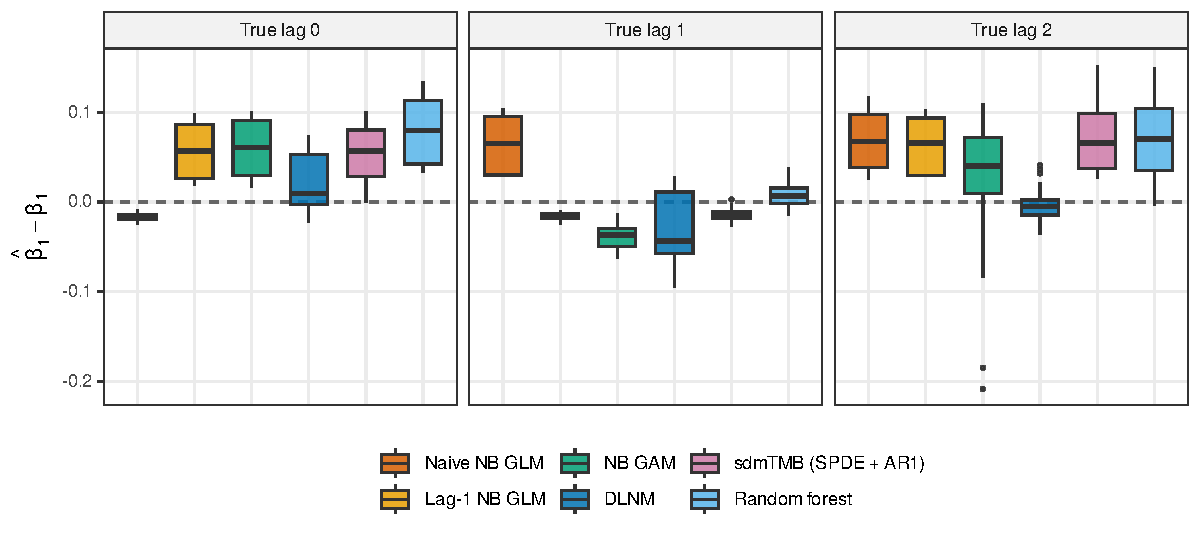
\includegraphics[width=\textwidth]{fig_bias_by_lag}
\caption{Mean bias of the estimated exposure coefficient, $\hat\beta_1 - \beta_1$, across the \nScenarios{} scenarios, by model class and true response lag. Each box summarises one third of the scenarios. The dashed line marks zero bias. Colours identify model classes and are used consistently in all figures.}
\label{fig:bias}
\end{figure}
\begin{figure}[H]\centering
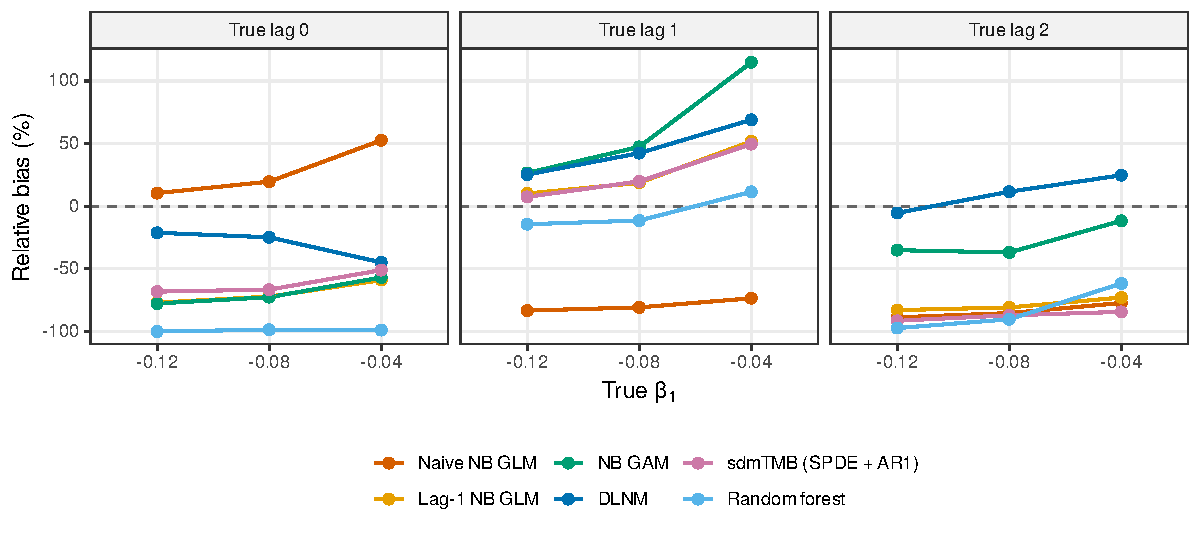
\includegraphics[width=\textwidth]{fig_relative_bias}
\caption{Relative bias, $100(\hat\beta_1-\beta_1)/\beta_1$, by true effect size and true lag. Negative values indicate under estimation of the magnitude of a negative effect.}
\label{fig:relbias}
\end{figure}

The lag aware GLM corrected the problem only when its assumed lag was the true one. At a one year lag its bias was \lagoneBiasLagOne{} (\lagoneRelBiasLagOne{}\% relative), but at zero and two years it collapsed in the same way as the naive model, under estimating by \lagoneRelBiasWrongLag{} respectively. Specifying a lag is therefore not a safeguard unless the lag is known, which in the reviewed literature it rarely was. The GAM, which also conditions on one year lagged exposure, showed the same dependence on the assumed lag.

The distributed lag model behaved differently. Because it estimates the lag profile rather than assuming it, its bias did not switch sign or magnitude with the true lag: \dlnmBiasLagZero{}, \dlnmBiasLagOne{} and \dlnmBiasLagTwo{} at lags of zero, one and two years, with relative bias between \dlnmRelBiasLagZero{}\% and \dlnmRelBiasLagOne{}\%. That robustness came at a cost in precision. The across replicate standard deviation of its estimate at a one year lag was \dlnmSdLagOne{}, against \lagoneSdLagOne{} for the correctly lagged GLM, and its RMSE at that lag (\dlnmRmseLagOne{}) exceeded the correctly lagged GLM's (\lagoneRmseLagOne{}). The practical trade is between an estimator that is accurate only if an unverifiable assumption holds and one that is less precise but does not fail when the assumption is wrong.

\subsubsection{Linear models produce confident intervals around the wrong value}\label{sec:res-coverage}

Nominal 95\% intervals from the two linear GLMs covered the true coefficient in \linearCoverageRange{} of scenarios (Fig.~\ref{fig:coverage}). The failure was not confined to the misspecified lag. Even at the correct lag, where the lag aware GLM's bias was only \lagoneBiasLagOne{}, its coverage was \lagoneCoverageCorrectLag{}, because the small bias induced by the unmodelled quadratic term is large relative to a standard error computed from several hundred site years. The intervals are correctly computed for the fitted model; they are centred on an estimate that the model cannot move to the right place. The GAM, which can represent the curvature, reached \gamCoverageLagOne{} coverage at the correct lag but fell to \gamCoverageMin{} when the lag was wrong. The DLNM's coverage ranged from \dlnmCoverageMin{} to \dlnmCoverageMax{} across lags (mean \dlnmCoverage{}), below nominal but an order of magnitude above the linear models. No class achieved nominal coverage in every condition, which argues for reporting the coverage behaviour of the chosen model under simulated conditions resembling the study rather than assuming it.

\begin{figure}[H]\centering
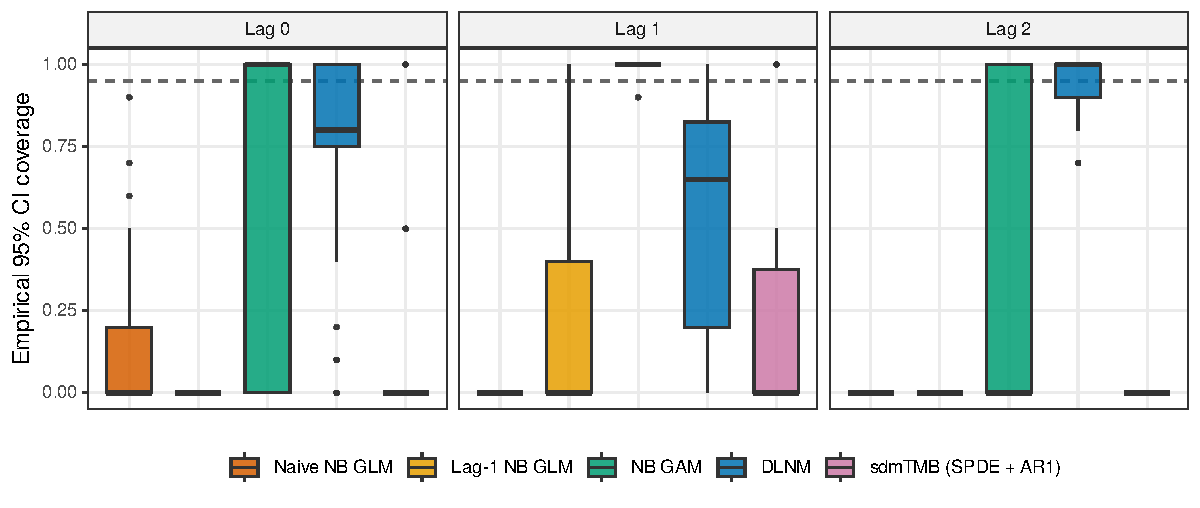
\includegraphics[width=\textwidth]{fig_coverage}
\caption{Empirical coverage of nominal 95\% confidence intervals for $\beta_1$, by model class and true lag. The dashed line marks nominal coverage. The random forest returns no interval and is omitted.}
\label{fig:coverage}
\end{figure}

\subsubsection{The best estimator is not the best predictor}\label{sec:res-prediction}

Held out predictive performance ordered the models differently from coefficient recovery (Fig.~\ref{fig:infpred}). Averaged across all scenarios the naive GLM, with the worst coefficient recovery at non zero lags, produced the highest held out log score (\naiveLogScore{}), followed by the random forest (\rfLogScore{}), the lag aware GLM (\lagoneLogScore{}) and the GAM (\gamLogScore{}). The ordering is driven by the contemporaneous scenarios, where the naive model is correctly specified and predicts well (\naiveLsLagZero{} against \lagoneLsLagZero{} for the lag aware GLM); at a one year lag the lag aware GLM and the GAM predicted better (\lagoneLsLagOne{} and \gamLsLagOne{} against \naiveLsLagOne{}). The random forest, which returns no interpretable coefficient, predicted competitively at every lag and its finite difference effect at a one year lag was nearly unbiased (\rfBiasLagOne{}), although without an interval. The quasi Poisson DLNM has no proper predictive density and was excluded from this comparison. A study that reports a single model cannot show both properties, and the model that would be chosen for prediction is not the one that would be chosen for attribution.

\begin{figure}[H]\centering
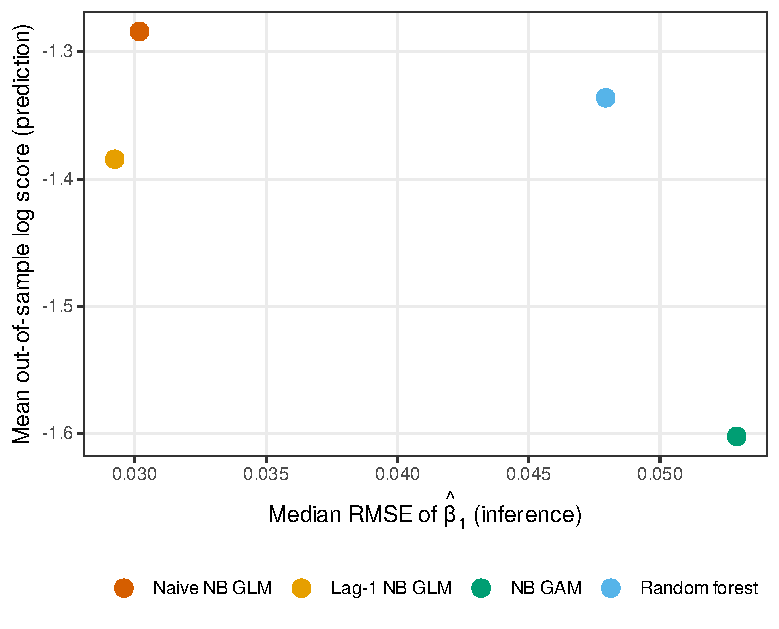
\includegraphics[width=0.6\textwidth]{fig_inference_prediction}
\caption{Coefficient recovery (median RMSE of $\hat\beta_1$ across scenarios) against held out predictive performance (mean negative binomial log predictive density of the final three years), one point per model class. The distributed lag model has no proper predictive density under the quasi Poisson fit and is omitted.}
\label{fig:infpred}
\end{figure}

\subsubsection{Region, grid size and spatial range do not change the ordering}\label{sec:res-region}

The ranking of model classes by absolute bias at a one year lag was \regionRankInvariant{} across the three regions (Fig.~\ref{fig:region}, Online Resource 1, Table S10). The naive GLM's bias at that lag ranged only from \naiveBiasLagOneRegionRange{} across Western Australia, the Northwest Atlantic and the Mediterranean, despite regional exposure distributions whose means differ by more than a factor of two. Grid size and spatial correlation range had no detectable effect on bias for any class (Online Resource 1, Table S11), which is expected because the fixed effect does not depend on the spatial field and the site fixed effects or random effects absorb the correlated noise. Residual Moran's $I$ of site mean residuals was small and negative for all regression classes (\moransIndep{} on independent panels and \moransCorr{} on correlated panels, averaged over models; Online Resource 1, Fig.~S6), confirming that in this design the spatial structure in exposure does not leave residual spatial dependence that a spatial random field would be needed to absorb. The lag problem is therefore not a regional artefact, and it is not alleviated by more sites.

\begin{figure}[H]\centering
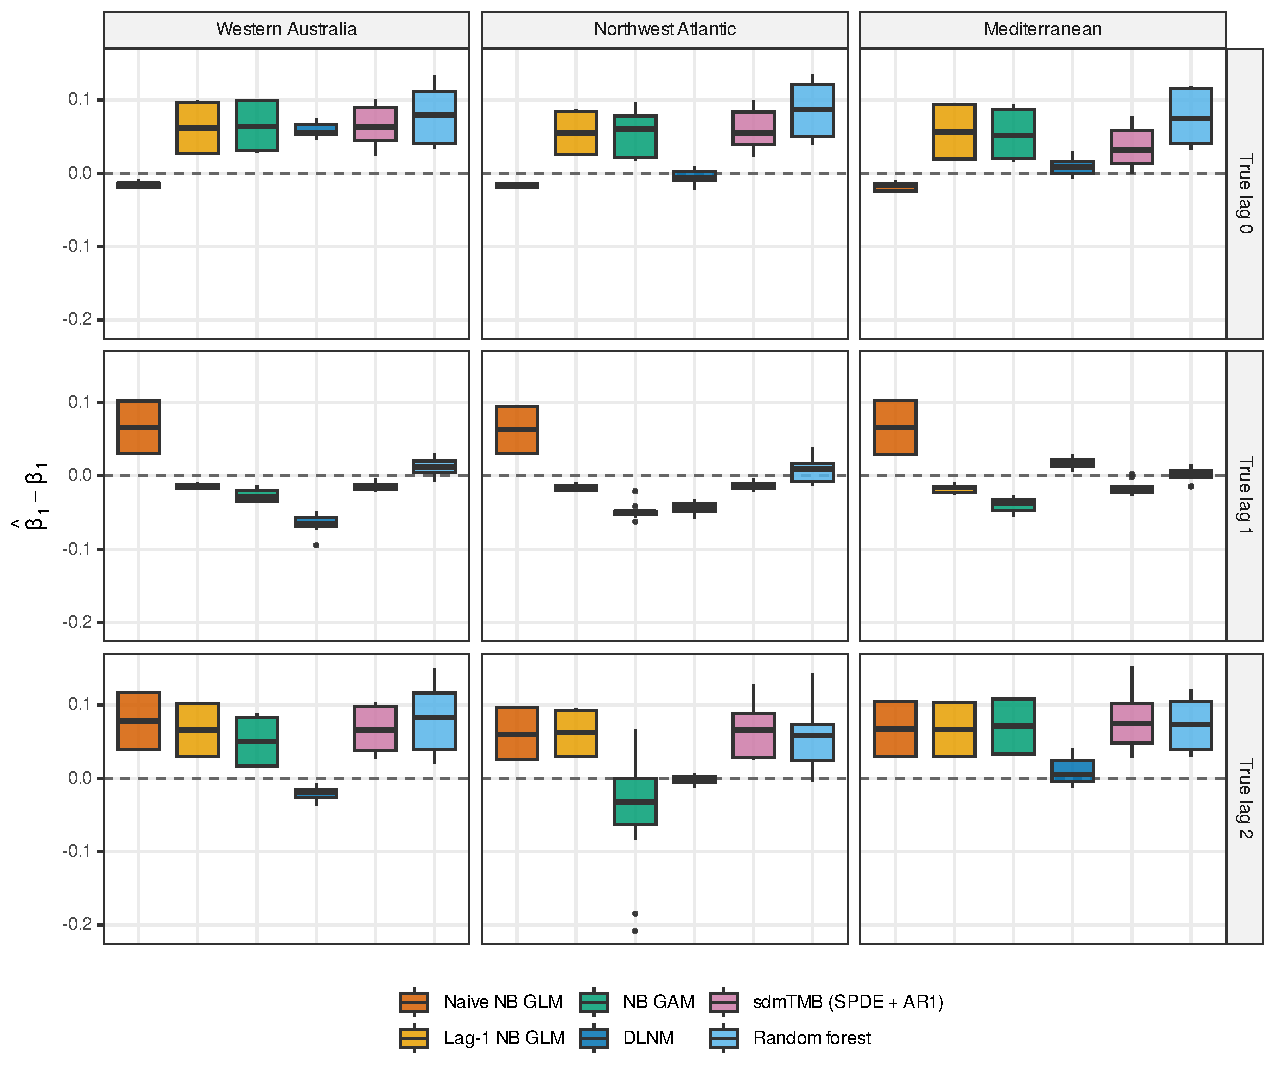
\includegraphics[width=\textwidth]{fig_region}
\caption{Mean bias of the estimated exposure coefficient by region, model class and true lag.}
\label{fig:region}
\end{figure}

\subsubsection{The spatial random field model}\label{sec:sdmtmb}

On the \sdmtmbPanelsN{} panels completed (\sdmtmbFits{} fits), sdmTMB returned point estimates whose bias (\sdmtmbBiasLagZero{}, \sdmtmbBiasLagOne{} and \sdmtmbBiasLagTwo{} at lags of zero, one and two years) tracked the lag aware GLM, as expected for a model that conditions on the same one year lagged covariate. Its \texttt{sanity()} diagnostic flagged \sdmtmbNonConvPct{}\% of fits, most often for a non positive definite Hessian (\sdmtmbNonConvIndep{}\% on spatially independent panels, \sdmtmbNonConvCorr{}\% on correlated ones), and interval coverage was \sdmtmbCoverage{}. These outcomes follow from the design rather than from a defect in the model. Equation~\ref{eq:dgp} contains no latent spatial field in the response; the only spatial structure is correlation among the site exposure series, and the site effects in the fixed effect models absorb it, as the near zero residual Moran's $I$ confirms. sdmTMB is therefore estimating a spatial variance and a spatiotemporal variance that are both truly zero, which places the optimiser at a boundary and is exactly the condition under which the package's documentation warns that the Hessian will be flagged. The design can show that a spatial random field model does not rescue a mis specified lag structure, and that its diagnostics report the absence of a field honestly; it cannot show the conditions under which such a model recovers a spatially varying effect, which would require a different data generating process (Section~\ref{sec:discussion}). Median fitting time was \sdmtmbMedianSec{}\,s per fit, against \naiveSec{}\,s for the GLM, which is the practical reason the model was run on a subset of the design.
